\let\negmedspace\undefined
\let\negthickspace\undefined
\documentclass[journal]{IEEEtran}
\usepackage[a5paper, margin=10mm, onecolumn]{geometry}
\usepackage{tfrupee} 

\setlength{\headheight}{1cm}
\setlength{\headsep}{0mm} 

\usepackage{gvv-book}
\usepackage{gvv}
\usepackage{amsmath,amssymb,amsfonts,amsthm}
\usepackage{algorithmic}
\usepackage{graphicx}
\usepackage{textcomp}
\usepackage{xcolor}
\usepackage{txfonts}
\usepackage{listings}
\usepackage{enumitem}
\usepackage{mathtools}
\usepackage{gensymb}
\usepackage{comment}
\usepackage[breaklinks=true]{hyperref}
\usepackage{tkz-euclide} 
\usepackage{listings}
\def\inputGnumericTable{}                      
\usepackage[latin1]{inputenc}                                
\usepackage{color}                                         
 
   
\usepackage{array}                                            
\usepackage{longtable}                                       
\usepackage{calc}              
 
                               
\usepackage{multirow}                                         
\usepackage{hhline}                            
 
               
\usepackage{ifthen}                                           
\usepackage{lscape}
\usepackage{tikz}
\usetikzlibrary{patterns}
\begin{document}


\vspace{3cm}


\title{GATE 2016 - General Aptitude \& Ecology (EY)}
\author{ee25btech11034 - Kishora Karthik}
\maketitle

{\let\newpage\relax\maketitle}

\renewcommand{\thefigure}{\theenumi}
\renewcommand{\thetable}{\theenumi}
\setlength{\intextsep}{10pt} 

\section*{\textbf{General Aptitude}}
\textbf{1) to 5) carry one mark each.}
 
\begin{enumerate}
    \item If I were you, I \underline{\hspace{3cm}} that laptop. It's much too expensive.
    \begin{multicols}{2}
    \begin{enumerate}
        \item won't buy
        \item shan't buy
        \item wouldn't buy
        \item would buy
    \end{enumerate}
    \end{multicols}
\hfill{(GATE EY 2016)}

    \item He turned a deaf ear to my request. What does the underlined phrasal verb mean?
    \begin{multicols}{4}
    \begin{enumerate}
        \item ignored
        \item appreciated
        \item twisted
        \item returned
    \end{enumerate}
    \end{multicols}
\hfill{(GATE EY 2016)}

    \item Choose the most appropriate set of words from the options given below to complete the following sentence. \underline{\hspace{2cm}} is a will, \underline{\hspace{2cm}} is a way.
    \begin{multicols}{2}
    \begin{enumerate}
        \item Wear, there, their
        \item Were, their, there
        \item Where, there, there
        \item Where, their, their
    \end{enumerate}
    \end{multicols}
\hfill{(GATE EY 2016)}

    \item $\brak{x\%\ \text{of}\ y}$ + $\brak{y\%\ \text{of}\ x}$ is equivalent to
    \begin{multicols}{4}
    \begin{enumerate}
        \item $2$\% of xy
        \item $2$\% of $\brak{\frac{xy}{100}}$
        \item xy\% of $100$
        \item $100$\% of xy
    \end{enumerate}
    \end{multicols}
\hfill{(GATE EY 2016)}

    \item The sum of the digits of a two digit number is $12$. If the new number formed by reversing the digits is greater than the original number by $54$, find the original number.
    \begin{multicols}{2}
    \begin{enumerate}
        \item $39$
        \item $57$
        \item $66$
        \item $93$
    \end{enumerate}
    \end{multicols}
\hfill{(GATE EY 2016)}

\textbf{Q.6 to Q.10 carry two marks each.}
 

\item Two finance companies, P and Q, declared fixed annual rates of interest on the amounts invested with them. The rates of interest offered by these companies may differ from year to year. Year-wise annual rates of interest offered by these companies are shown by the line graph provided below.
\begin{figure}
    \centering
    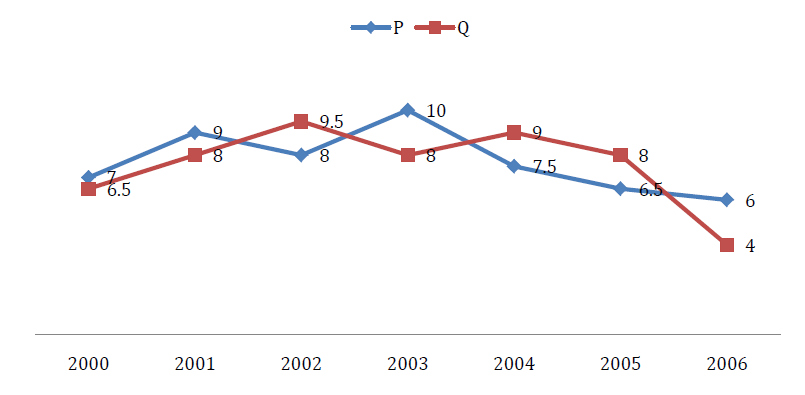
\includegraphics[width=0.7\columnwidth]{figs/Q-6.png}
    \caption{Interest rates for companies P and Q from 2000 to 2006}
    \label{Fig.1}
\end{figure}
If the amounts invested in the companies, P and Q, in $2006$ are in the ratio $8$:$9$, then the amounts received after one year as interests from companies P and Q would be in the ratio:
\begin{multicols}{2}
\begin{enumerate}
    \item $2$:$3$
    \item $3$:$4$
    \item $6$:$7$
    \item $4$:$3$
\end{enumerate}
\end{multicols}
\hfill{(GATE EY 2016)}

\item Today, we consider Ashoka as a great ruler because of the copious evidence he left behind in the form of stone carved edicts. Historians tend to correlate greatness of a king at his time with the availability of evidence today. Which of the following can be logically inferred from the above sentences?
\begin{enumerate}
    \item Emperors who do not leave significant sculpted evidence are completely forgotten.
    \item Ashoka produced stone carved edicts to ensure that later historians will respect him.
    \item Statues of kings are a reminder of their greatness.
    \item A king's greatness, as we know him today, is interpreted by historians.
    \end{enumerate}
\hfill{(GATE EY 2016)}

\item Fact 1: Humans are mammals. \\
Fact 2: Some humans are engineers. \\
Fact 3: Engineers build houses.
\\
If the above statements are facts, which of the following can be logically inferred? 
  \begin{enumerate}[label=\Roman*.]
    \item All mammals build houses. 
    \item  Engineers are mammals. 
    \item Some humans are not engineers.
  \end{enumerate}
\begin{multicols}{2}
\begin{enumerate}
    \item II only.
    \item III only.
    \item I, II and III.
    \item I only.
    \end{enumerate}
\end{multicols}
\hfill{(GATE EY 2016)}

\item A square pyramid has a base perimeter $x$, and the slant height is half of the perimeter. What is the lateral surface area of the pyramid?
\begin{multicols}{4}
\begin{enumerate}
    \item $x^{2}$
    \item $0.75 x^{2}$
    \item $0.50 x^{2}$
    \item $0.25 x^{2}$
\end{enumerate}
\end{multicols}
\hfill{(GATE EY 2016)}

\item Ananth takes $6$ hours and Bharath takes $4$ hours to read a book. Both started reading copies of the book at the same time. After how many hours is the number of pages to be read by Ananth, twice that to be read by Bharath? Assume Ananth and Bharath read all the pages with constant pace.
\begin{multicols}{4}
\begin{enumerate}
    \item $1$
    \item $2$
    \item $3$
    \item $4$
\end{enumerate}
\end{multicols}
\hfill{(GATE EY 2016)}

\end{enumerate}
\bigskip
\centering {\textbf{\large{END OF QUESTION PAPER}}}

\clearpage

\section*{\textbf{Ecology (EY)}}
\begin{flushleft}
\textbf{1) to 25) carry one mark each.}
    \end{flushleft}
\begin{enumerate}

\item Different kinds of limbs, such as the wings of birds and bats, and the flippers of turtles, whales and dolphins, have the same underlying skeletal structure. This is an example of:
\begin{multicols}{4}
\begin{enumerate}
    \item Analogy
    \item Convergence
    \item Homology
    \item Genetic drift
\end{enumerate}
\end{multicols}
\hfill{(GATE EY 2016)}

\item Forests with a high density of native conifer trees are found in:
\begin{multicols}{2}
\begin{enumerate}
    \item Gujarat
    \item Haryana
    \item Himachal Pradesh
    \item Odisha
\end{enumerate}
\end{multicols}
\hfill{(GATE EY 2016)}

\item Ozone layer depletion, since the 1970s, is primarily attributed to:
\begin{multicols}{2}
\begin{enumerate}
    \item carbon dioxide
    \item chlorofluorocarbons
    \item global warming
    \item UV radiation
\end{enumerate}
\end{multicols}
\hfill{(GATE EY 2016)}

\item The evolution of the amniotic egg in reptiles allowed them to:
\begin{enumerate}
    \item colonize dry terrestrial environments
    \item give birth to live young
    \item lay eggs in water and on land
    \item live in aquatic environments
\end{enumerate}
\hfill{(GATE EY 2016)}

\item Which of the following phyla are most closely related to chordates?
\begin{multicols}{4}
\begin{enumerate}
    \item Annelida
    \item Arthropoda
    \item Echinodermata
    \item Mollusca
\end{enumerate}
\end{multicols}
\hfill{(GATE EY 2016)}

\item Limb lengths were measured for $50$ individuals from a population of lizards and the sample variance was calculated to be $64$ $cm^{2}$. The standard deviation for this sample is \underline{\hspace{3cm}} cm.

\hfill{(GATE EY 2016)}

\item Most terrestrial ecosystems have a pyramidal structure of standing biomass across trophic levels where biomass of producers $>$ primary consumers $>$ secondary consumers $>$ tertiary consumers. However, some aquatic ecosystems have an inverted pyramidal structure where the standing biomass of producers $<$ primary consumers. An explanation for this is:
\begin{enumerate}
    \item greater efficiency of primary consumers in aquatic ecosystems
    \item high turnover rates of aquatic producers relative to consumers
    \item low nutrient concentrations in aquatic ecosystems
    \item very high light limitation in aquatic ecosystems
\end{enumerate}
\hfill{(GATE EY 2016)}

\item In an experiment, a PhD student found that the traits, flower colour and seed size, did not follow Mendel's Law of Independent Assortment. A possible explanation for this observation is:
\begin{multicols}{2}
\begin{enumerate}
    \item co-dominance between alleles
    \item incomplete dominance
    \item linkage between the traits
    \item loci on different chromosomes
\end{enumerate}
\end{multicols}
\hfill{(GATE EY 2016)}

\item Which of the following invertebrates has the lowest gut length:body length ratio?
\begin{multicols}{4}
\begin{enumerate}
    \item dragonflies
    \item grasshoppers
    \item leaf hoppers
    \item termites
\end{enumerate}
\end{multicols}
\hfill{(GATE EY 2016)}

\item Allopatric speciation occurs when two populations diverge because of geographical separation. Rates of allopatric speciation are likely to be higher in:
\begin{enumerate}
    \item marine organisms with active dispersal
    \item marine organisms with passive dispersal
    \item terrestrial organisms with high dispersal ability
    \item terrestrial organisms with low dispersal ability
\end{enumerate}
\hfill{(GATE EY 2016)}

\item For nearly $200$ years, biogeographers have noted that the tropics have more terrestrial species than temperate regions. Which of the following is NOT a plausible explanation for this pattern?
\begin{enumerate}
    \item Diversification rates are higher in the tropics
    \item Energy inputs are higher in the tropics
    \item There is greater land area in the tropics
    \item Tropical species have greater climatic tolerance
\end{enumerate}
\hfill{(GATE EY 2016)}

\item If the rate of non-synonymous substitution at a locus exceeds that of synonymous substitution, then:
\begin{enumerate}
    \item deleterious mutations are accumulating
    \item evolution is not occurring
    \item genetic drift is operating
    \item selection is operating
\end{enumerate}

\hfill{(GATE EY 2016)}

\item There are $N$ individuals in a haploid population. At a given locus, there are $2$ alleles, AL1 and AL2. The number of copies of allele AL1 is $Z1$, and the number of copies of allele AL2 is $Z2$ in the population. What is the frequency of allele AL2?
\begin{multicols}{4}
\begin{enumerate}
    \item $\frac{Z1}{N}$
    \item $\frac{Z2}{N}$
    \item $Z1+Z2$
    \item $\frac{(Z1+Z2)}{N}$
\end{enumerate}
\end{multicols}
\hfill{(GATE EY 2016)}

\item According to Hamilton's Rule, an altruistic act will spread in a population due to kin selection, when $\frac{B}{C} > \frac{1}{r}$, where B is the benefit to the recipient, C is the cost to the actor and r is the genetic relatedness of the recipient to the actor. Given this relationship, a human may forego producing one of her own offspring to help her full sibling raise offspring, only if it results in at least \underline{\hspace{1cm}} or more extra offspring produced by her sibling.
\begin{multicols}{4}
\begin{enumerate}
    \item $1$
    \item $2$
    \item $4$
    \item $8$
\end{enumerate}
\end{multicols}
\hfill{(GATE EY 2016)}

\item Which of the following is NOT a plant hormone?
\begin{multicols}{4}
\begin{enumerate}
    \item Corticosterone
    \item Ethylene
    \item Jasmonic acid
    \item Salicylic acid
\end{enumerate}
\end{multicols}
\hfill{(GATE EY 2016)}

\item Among foraging shore birds, feeding rates ($F$, number of prey items consumed in $5$ minutes) decrease as the number of neighbours ($N$) increases as follows: $F = 10 - 0.9N$. The maximum feeding rate is \underline{\hspace{3cm}}.

\hfill{(GATE EY 2016)}

\item Which of the following is NOT an adaptation to reduce the risk of predation?
\begin{multicols}{2}
\begin{enumerate}
    \item Alarm calling
    \item Cannibalism
    \item Group living
    \item Sentinel behaviour
\end{enumerate}
\end{multicols}
\hfill{(GATE EY 2016)}

\item Which of the following is NOT an example of an evolutionary arms race?
\begin{enumerate}
    \item Brood parasite and host interactions
    \item Conflict between parents and offspring
    \item Predator and prey interactions
    \item Recognition between kin
\end{enumerate}
\hfill{(GATE EY 2016)}

\item The Weber-Fechner law states that the magnitude of a perceived sensation increases as $\log_{10}$ of stimulus intensity. Let us assume a background stimulus level of $1$ unit, which increases to $10$ units in situation P and to $100$ units in situation Q. The perceived sensation in situation Q is stronger than the sensation perceived in situation P by a factor of \underline{\hspace{3cm}}.
\hfill{(GATE EY 2016)}

\item Monotremes are unique among mammals because they:
\begin{multicols}{2}
\begin{enumerate}
    \item have claws
    \item lay eggs
    \item possess hair
    \item produce milk
\end{enumerate}
\end{multicols}
\hfill{(GATE EY 2016)}

\item The most important reason for a neuron to be myelinated is to:
\begin{enumerate}
    \item decrease the possibility of excitation from nearby muscle activity
    \item increase the diameter of the axon to slow down the action potential
    \item increase the speed of an action potential
    \item protect the nerve from physical damage
\end{enumerate}
\hfill{(GATE EY 2016)}

\item A small isolated population is more likely to undergo speciation than a large population because, compared to the large population, the small population:
\begin{multicols}{2}
\begin{enumerate}
    \item has greater genetic diversity
    \item has a higher mutation rate
    \item is more affected by genetic drift
    \item is more susceptible to gene flow
\end{enumerate}
\end{multicols}
\hfill{(GATE EY 2016)}

\item To which of the following families do the important timber species, sal and teak, belong? 
    \begin{enumerate}[label=(\roman*)]
        \item Dipterocarpaceae
        \item Poaceae
        \item Solanaceae
        \item Verbenaceae
    \end{enumerate}
\begin{multicols}{4}
\begin{enumerate}
    \item i and ii
    \item i and iv
    \item ii and iii
    \item iii only
\end{enumerate}
\end{multicols}
\hfill{(GATE EY 2016)}

\item The yields of which of these crops are most likely to be reduced by ongoing declines in bee populations?
\begin{multicols}{4}
\begin{enumerate}
    \item coffee
    \item rice
    \item tea
    \item wheat
\end{enumerate}
\end{multicols}
\hfill{(GATE EY 2016)}

\item Dichlorodiphenyltrichloroethane is related to the phenomenon of:
\begin{enumerate}
    \item biomagnification in food webs
    \item coral bleaching in oceans
    \item the greenhouse effect
    \item ozone layer depletion
\end{enumerate}
\hfill{(GATE EY 2016)}

\textbf{Q.26 to Q.55 carry two marks each.}

\item Here is a data set on wing lengths in cm: $8$, $9$, $10$, $10$, $12$, $13$, $13$, $14$, $15$, $15$, $15$, $19$, $22$, $25$, $25$. For this sample data set, the mean, median and mode are \underline{\hspace{3cm}}, \underline{\hspace{3cm}} and \underline{\hspace{3cm}} respectively.
\begin{multicols}{4}
\begin{enumerate}
    \item $15$, $8$ and $25$
    \item $15$, $14$ and $8$
    \item $15$, $14$ and $15$
    \item $15$, $15$ and $15$
\end{enumerate}
\end{multicols}
\hfill{(GATE EY 2016)}

\item Dragonflies eat plant pollinators. Fish eat dragonfly larvae. A study compared the fitness of plants growing near ponds with and without fish. Given the above set of trophic interactions in a community, this study will likely find that:
\begin{enumerate}
    \item the fitness of plants is not affected by dragonflies
    \item the fitness of plants is not affected by whether ponds have fish
    \item plants growing near ponds without fish have higher fitness
    \item plants growing near ponds with fish have higher fitness
\end{enumerate}
\hfill{(GATE EY 2016)}

\item Which of the following statements CANNOT be inferred from the following phylogenetic tree? 
\begin{figure}[!ht]
    \centering
    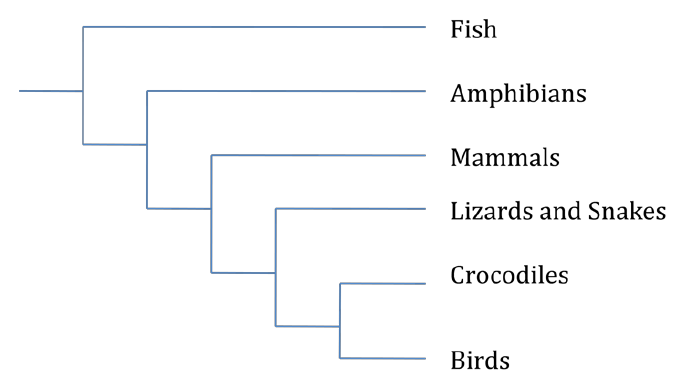
\includegraphics[width=0.7\columnwidth]{figs/Q-28.png}
    \caption{}
    \label{}
\end{figure}
\begin{enumerate}
    \item Crocodiles are more closely related to birds than to the other reptiles
    \item Fish, lizards and snakes have a common ancestor
    \item Mammals and reptiles have evolved from amphibians
    \item Mammals are more closely related to crocodiles than to amphibians
\end{enumerate}
\hfill{(GATE EY 2016)}

\item Assume that the abundance of a species in a community is proportional to the size of its niche. As each new species colonises this community, an existing niche is split. The resultant relative abundances of species in this community will be most \underline{uneven} if:
\begin{enumerate}
    \item The largest niche is always split when a new species colonises
    \item The niches are split at random, independent of their size
    \item The probability of a niche being split is proportional to its size
    \item The smallest niche is always split when a new species colonises
\end{enumerate}
\hfill{(GATE EY 2016)}

\item To study colour preference in bees, a student uses artificial flowers with a sugar reward. She gives bees a choice between blue round flowers and yellow square flowers of the same size. She finds that bees choose the blue flowers significantly more often than the yellow flowers and concludes that bees have a colour preference for blue flowers. However, her friend disagrees and suggests that she should have done the experiment differently. Which of the following would have been more appropriate to test for colour preference in bees?
\begin{enumerate}
    \item choice between blue round and blue square flowers
    \item choice between blue round and yellow round flowers
    \item choice between yellow round and blue square flowers
    \item choice between yellow round and yellow square flowers
\end{enumerate}
\hfill{(GATE EY 2016)}

\item Which of the following does NOT form a component of phytohormone action?
\begin{multicols}{2}
\begin{enumerate}
    \item recognition of specific proteins
    \item regulation of gene activity
    \item splitting of water molecules
    \item signal transduction across the cell
\end{enumerate}
\end{multicols}
\hfill{(GATE EY 2016)}

\item The following three panels show the change in population size over time for two species when they are found alone and when they are found together. Which kind of interaction best describes the relationship between the two species? 
\begin{figure}[!ht]
    \centering
    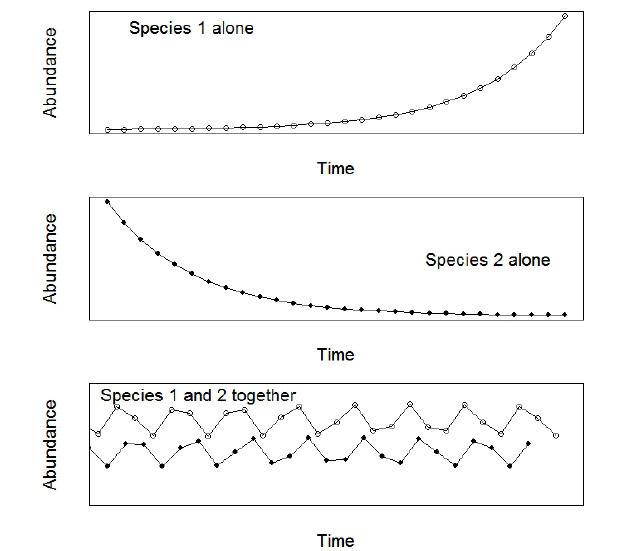
\includegraphics[width=0.7\columnwidth]{figs/Q-32.png}
    \caption{Relation between abundance and time}
    \label{Fig.2}
\end{figure}
\begin{multicols}{4}
\begin{enumerate}
    \item Amensalism
    \item Competition
    \item Mutualism
    \item Predation
\end{enumerate}
\end{multicols}
\hfill{(GATE EY 2016)}

\item Fresh water fish belonging to the family Galaxoidae are found exclusively in the southern parts of the continents of South America, Africa and Australia. This pattern is explained by the theory proposed by:
\begin{multicols}{2}
\begin{enumerate}
    \item Alfred Russel Wallace
    \item Alfred Wegener
    \item Charles Darwin
    \item Charles Lyell
\end{enumerate}
\end{multicols}
\hfill{(GATE EY 2016)}

\item Ant species X preys upon ant species Y. A researcher has the following set of observations regarding the behaviour of species X where aggression signifies a predatory response. \begin{center}
\begin{tabular}{ll}
    \textbf{Group I} & \textbf{Group II} \\
    P. Ferrite & 1. Hexagonal Close Packed (HCP) \\
    Q. Austenite & 2. Body Centered Cubic (BCC) \\
    R. Martensite & 3. Body Centered Tetragonal (BCT) \\
    & 4. Face Centered Cubic (FCC)
\end{tabular}
\end{center}
Which of the following statement(s) are correct regarding the behaviour of Species X?
\begin{enumerate}[label=(\roman*)]  
    \item A glass bead is sufficient to elicit the predatory response.
    \item Both chemical and non-chemical cues are involved in the predatory response.
    \item Chemical cues are necessary to elicit the predatory response.
    \item Chemical cues are sufficient to elicit the predatory response
\end{enumerate}

\begin{multicols}{2}
\begin{enumerate}
    \item i, ii
    \item ii, iv
    \item i, iii
    \item iii, iv
\end{enumerate}
\end{multicols}
\hfill{(GATE EY 2016)}

\item In the schematic below, the left panel represents climatic zones occupied by two different biomes, X and Y, along gradients of temperature and precipitation. The right panel depicts the expected species-area relationships of these two biomes. From the figs below, which of the following are most likely to be true?
\begin{enumerate}[label=(\roman*)]  
    \item Biome X will show pattern W
    \item Biome Y will show pattern Z
    \item Biome X will show pattern Z
    \item Biome Y will show pattern W
\end{enumerate}
\begin{figure}[!ht]
    \centering
    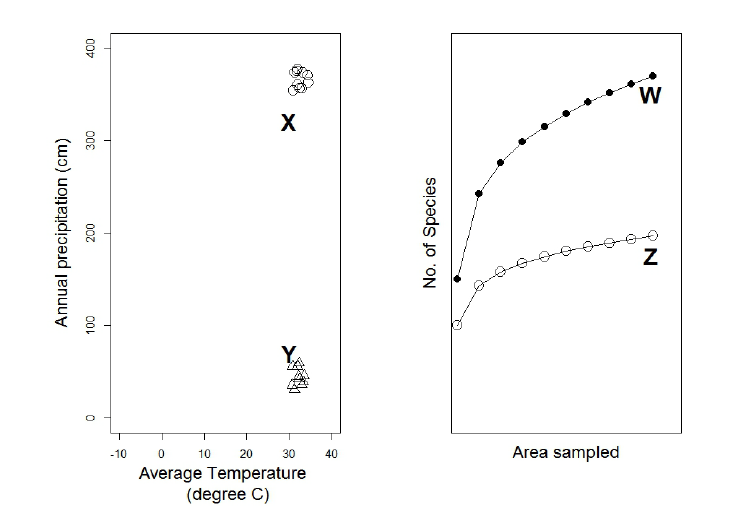
\includegraphics[width=0.2\columnwidth]{figs/Q-35.png}
    \caption{Climatic zones of biomes X and Y}
    \label{Fig.3}
\end{figure}
\begin{multicols}{2}
\begin{enumerate}
    \item i and ii
    \item i and iv
    \item ii and iii
    \item iii and iv
\end{enumerate}
\end{multicols}
\hfill{(GATE EY 2016)}

\item In many plant and animal communities that are found on islands, the number of species (S) changes with the area (A) of the island as follows: $S=cA^{z}$, where $0<z<1$ and $c>0$. Which of the following graphs best represents such a species-area relationship? 
\begin{figure}[!ht]
    \centering
    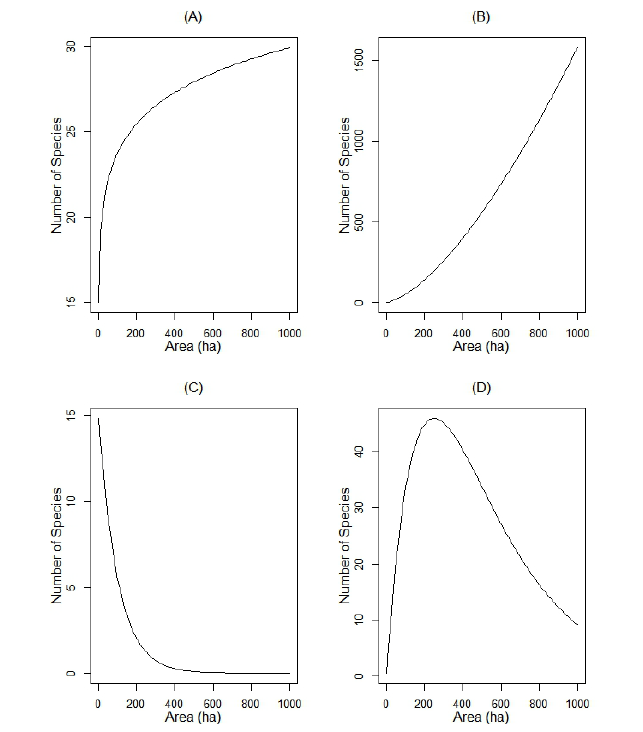
\includegraphics[width=0.7\columnwidth]{figs/Q-36.png}
    \caption{Graph of number of species varying with area}
    \label{Fig.4}
\end{figure}

\hfill{(GATE EY 2016)}

\item Males in a population differ in the time they spend displaying to females. A researcher hypothesizes that predators are responsible for these differences. Males display for longer durations when there are no predators in the vicinity and for shorter durations when there is a predator nearby. Which of the following study designs is the most appropriate test of this hypothesis?
\begin{enumerate}
    \item Map predator distribution in the area; measure the abundance of females;
quantify the natural variation in male display rates in areas without predators
    \item Measure display rates of males at the beginning of the breeding season;
remove all predators from the study site; then measure male display rates later in the breeding season;
repeat for multiple populations
    \item Measure display rates of males in areas with and without predators;
randomly assign males to two treatments: 
        \begin{enumerate}[label=(\roman*)]
        \item capture and release back in original area
        \item capture and switch between areas; measure display rates for all experimental males
    \end{enumerate}
    \item Measure display rates of males in areas with and without predators;
randomly assign males to two treatments:
        \begin{enumerate}[label=(\roman*)]
        \item addition of females to the area 
        \item removal of females from the area; measure display rates for all experimental males
    \end{enumerate} 
\end{enumerate}
\hfill{(GATE EY 2016)}

\item In Batesian mimicry, a harmless species mimics a harmful or toxic model species. Increasing the relative abundance of the mimic will:
\begin{enumerate}
    \item negatively affect both model and mimic populations
    \item negatively affect the model but not the mimic population
    \item positively affect both model and mimic populations
    \item positively affect the mimic but not the model population
\end{enumerate}
\hfill{(GATE EY 2016)}

\item There are two alleles at a locus in a population in Hardy-Weinberg equilibrium. If the proportion of the dominant phenotype is $0.99$, what proportion of the population is heterozygous? \underline{\hspace{3cm}}.
\hfill{(GATE EY 2016)}

\item Haemophilia is a condition resulting from a sex-linked recessive gene in which individuals can suffer from excessive bleeding due to a blood-clotting disorder. In a human family with three children, the two sons are afflicted with haemophilia while the parents are normal. The probability that the daughter has inherited the gene for haemophilia is \underline{\hspace{1cm}}, and the probability that she is afflicted by haemophilia is \underline{\hspace{1cm}}.
\begin{multicols}{2}
\begin{enumerate}
    \item $1/2$, $0$
    \item $1/2$, $1$
    \item $1/2$, $1/4$
    \item $1/4$, $0$
\end{enumerate}
\end{multicols}
\hfill{(GATE EY 2016)}

\item Which of the graphs below represents the relationship between population size ($N$) and population growth rate ($\frac{dN}{dt}$) for a population showing exponential growth? 
\begin{figure}[h]
    \centering
    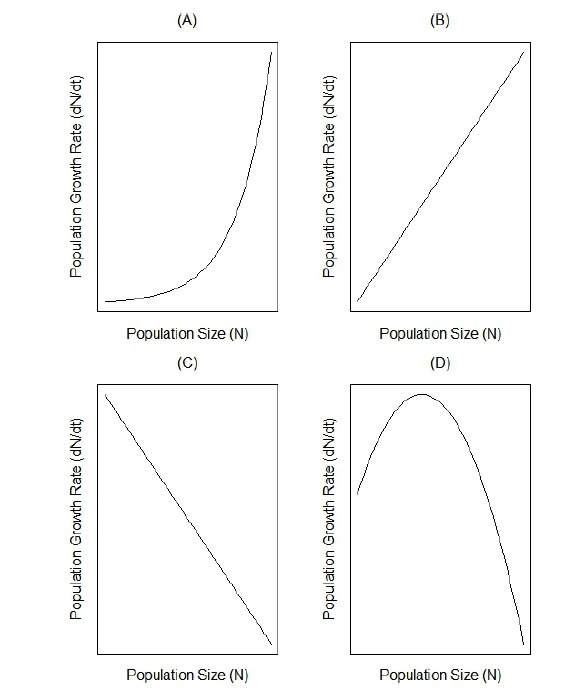
\includegraphics[width=0.1\columnwidth]{figs/Q-41.png}
    \caption{Population Growth Rate v/s Population Size}
    \label{Fig.5}
\end{figure}

\hfill{(GATE EY 2016)}

\item Two islands, P and Q, are similar in habitat and other features. They are $100$ and $200$ km$^2$ in size respectively, but have the same number of species. Which of the following statements can independently explain this observation?
    \begin{enumerate}[label=(\roman*)]
        \item  P is closer to the mainland than Q
        \item P is further away from the mainland than Q
        \item P has higher speciation rates than Q
        \item P has lower speciation rates than Q
    \end{enumerate}
\begin{multicols}{4}
\begin{enumerate}
    \item i and iv
    \item i and iii
    \item ii and iii
    \item ii and iv
\end{enumerate}
\end{multicols}
\hfill{(GATE EY 2016)}

\item In reverse sexual selection, variance in mating success is higher in females than in males. In such species, which of the following is most expected?
\begin{enumerate}
    \item Females are the competing sex and males are the choosy sex
    \item Males are the competing sex and females are the choosy sex
    \item Mating is random and both sexes are not choosy
    \item Mating is non-random and both sexes are equally choosy
\end{enumerate}
\hfill{(GATE EY 2016)}

\item According to the Hamilton-Zuk hypothesis, females prefer males with the most elaborate ornaments because those ornaments signal parasite resistance. Which of the following is NOT an assumption of this hypothesis?
\begin{enumerate}
    \item Parasites reduce male fitness
    \item Parasite resistance is indicated by male ornamentation
    \item Parasite resistance is genetic
    \item Parasite load is positively correlated with male ornamentation
\end{enumerate}
\hfill{(GATE EY 2016)}

\item A plant produces flowers that are open through the day and the night. An experimenter places pollen on the stigmas of freshly opened flowers and covers them after pollination to prevent natural pollinators from having access to the flowers. When experimental pollination was carried out during the day, $40$\% of the flowers yielded fruit. When experimental pollination was carried out during the night, $80$\% of the flowers yielded fruit. However, when flowers were kept open to natural pollination during the day (covered at night), $35$\% of flowers produced fruit. $20$\% of flowers exposed to natural pollination during the night (covered during the day) produced fruit. Which of the following statements is NOT a plausible explanation of these results?
\begin{enumerate}
    \item night pollinators are low in abundance
    \item night pollinators are abundant
    \item night pollinators are low in pollination efficiency
    \item pollinators are active during the day
\end{enumerate}
\hfill{(GATE EY 2016)}

\item Sex is determined by temperature in many reptiles, including crocodiles and turtles. While lower temperatures produce males in turtles, the pattern is the opposite in crocodiles. Due to climate change, there is an increase in temperatures which results in a change in sex ratios. In small populations, this change in demography is likely to negatively impact the population growth of:
\begin{enumerate}
    \item crocodiles more than turtles
    \item neither of the two species
    \item both species equally
    \item turtles more than crocodiles
\end{enumerate}
\hfill{(GATE EY 2016)}

\item An unbiased coin is tossed four times. What is the probability of getting at least three "heads" in a row? \underline{\hspace{3cm}}.
\hfill{(GATE EY 2016)}
\bigskip 
\item In a study of interactions between plants, ants and caterpillars, the following experimental treatments were imposed;
\begin{enumerate}[label=(\roman*)]
        \item Control (both ants and caterpillars are present
        \item Ant removal
        \item Caterpillar removal
        \item Ant and caterpillar removal
    \end{enumerate}
Plus ($+$) indicates presence and minus ($-$) indicates absence on plants. The results for plant performance (growth) from this experiment are shown in the figure below. Plant performance in all treatments were significantly different from each other. Based on these results, which of the following inferences is correct? 
\begin{figure}[!ht]
    \centering
    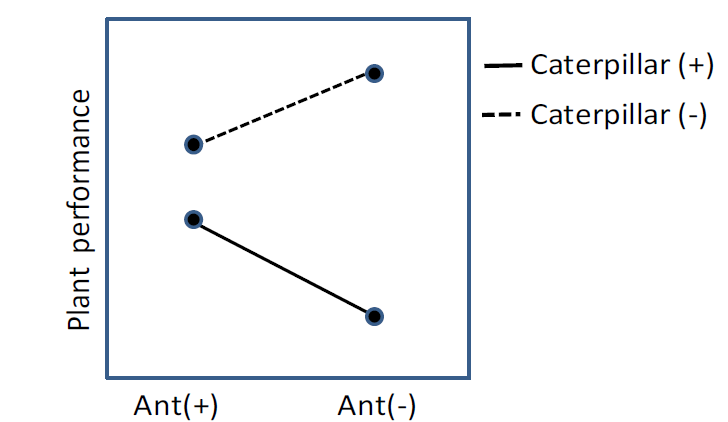
\includegraphics[width=0.5\columnwidth]{figs/Q-48.png}
    \caption{Interaction between plants, ants and caterpillars}
    \label{Fig.6}
\end{figure}
\begin{enumerate}
    \item In the absence of caterpillars, ants negatively affected plant performance
    \item In the absence of ants, caterpillars positively affected plant performance
    \item In the presence of caterpillars, ants negatively affected plant performance
    \item In the presence of ants, caterpillars positively affected plant performance
\end{enumerate}
\hfill{(GATE EY 2016)}

\item Both males and females of a fish species show variation in colour. A population of this species consists of $40$\% blue females, $20$\% red females, $20$\% blue males and $20$\% red males. A researcher catches one fish at random from this population. Given that a male fish is caught, the probability that it is blue is \underline{\hspace{3cm}}.
\hfill{(GATE EY 2016)}

 


\item Assume that an asexually propagating fungus has three colors of colonies, white, black and red. Such variability in color may have originated due to:
\begin{multicols}{2}
\begin{enumerate}
    \item germline mutation
    \item heterokaryosis
    \item genetic linkage
    \item sexual cross-over
\end{enumerate}
\end{multicols}
\hfill{(GATE EY 2016)}

\item Shannon's index of diversity is calculated using the equation below, where $p_i$ is the proportion of the $i^{th}$ species and ln is natural logarithm. For a community with a given number of species, which of the following statements is true?
$$ H = -\sum_{i=1}^{n} p_i \ln(p_i) $$
\begin{enumerate}
    \item Shannon's index will be highest if all species have equal abundance
    \item Shannon's index will be highest if one species is highly dominant
    \item Shannon's index will be highest if there are many rare species
    \item The relative abundance is irrelevant to Shannon's index
\end{enumerate}
\hfill{(GATE EY 2016)}

\item The schematic below shows the relationship between survivorship with age (relative to maximum lifespan) in Species 1 (dashed line) and Species 2 (solid line). Which of the following inferences is compatible with this figure? 
\begin{figure}[!ht]
    \centering
    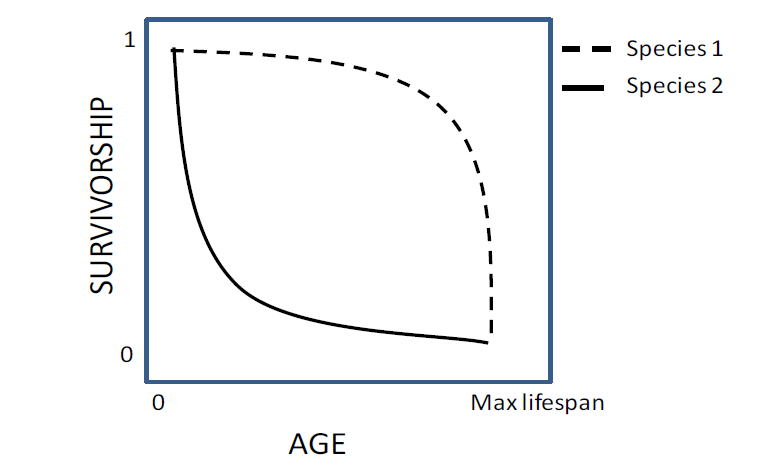
\includegraphics[width=0.7\columnwidth]{figs/Q-52.png}
    \caption{Relationship between survivorship with age}
    \label{Fig.7}
\end{figure}
\begin{enumerate}
    \item Species 1 is a mouse, Species 2 is an elephant
    \item Species 1 is a rat, Species 2 is a tree shrew
    \item Species 1 is a whale, Species 2 is a mouse
    \item Species 1 is a whale, Species 2 is an elephant
\end{enumerate}
\hfill{(GATE EY 2016)}

\item A team of conservation biologists, surveying a population of frogs on an island, captured and marked $312$ individuals in the first sample. In a second sampling, $3$ days later, the team caught $140$ individuals of which $26$ were previously marked. The total number of frogs on the island is estimated to be \underline{\hspace{3cm}}.
\hfill{(GATE EY 2016)}
\bigskip
 
\item The following equation represents a hypothetical relationship between fitness ($w$) and shoot:root ratio ($r$) in individuals of a plant species: $w = 10r - 10r^2$. At what value of shoot:root ratio ($r$), do these plants achieve maximum fitness? \underline{\hspace{3cm}}.
\hfill{(GATE EY 2016)}
\bigskip
 
\item The relative abundance of C3 relative to C4 plant species increases with latitude because of the associated temperature gradient. A study in North America found that at $42$\degree North, C3 plants become more abundant than C4 plants. Given an increase in mean global temperatures by $10$\degree C and no other changes in environmental conditions, the latitude at which C3 plants become more abundant:
\begin{enumerate}
    \item will move Northwards towards the polar region
    \item will move Southwards towards the equator
    \item will move South of the equator
    \item will not change in response to temperature
\end{enumerate}
\hfill{(GATE EY 2016)}

\end{enumerate}
\bigskip
\centering {\textbf{\large{END OF QUESTION PAPER}}}

\end{document}